\large{
Di seguito sono riportate tutte le tecnologie utilizzate, ognuna accompagnata da una descrizione, che a volte comprenderà anche un esempio di utilizzo e la motivazione che ha spinto ad utilizzare tale tecnologia. Oltre questo sono anche riportate tutte le metodologie applicate per poter realizzare il progetto.

\section{Visualizzazione delle informazioni}
L'intero lavoro svolto si basa su due importanti settori informatici quali la teoria dei grafi che abbiamo detto essere la disciplina che si occupa dello studio dei grafi e spesso di consentirne delle analisi in termini quantitativi e algoritmici, con basi di teoria della complessità, e la visualizzazione delle informazioni. Per quanto concerne quest'ultimo, può essere definito come l'utilizzo o comunque l'impiego di rappresentazioni visuali ed interattive di dati astratti con il compito di amplificarne la conoscenza degli stessi o anche come la comunicazione di dati attraverso l'utilizzo di interfacce visuali. Questo particolare settore è di grande rilievo sia per l'analisi dei dati che per la presentazione e quindi per la comunicazione degli stessi. Importante però è non assegnare alla visualizzazione delle informazioni il semplice scopo di creazione di grafici per scopi privi di informazione in quanto essa è la base su cui si andrà a lavorare. \\
Per quanto riguarda i dati astratti citati prima essi possono essere di due tipi, strutturati e non strutturati. I dati strutturati sono rigidamente formattati e si stima che siano soltato il 20\% dei dati che si producono e sono solitamente organizzati in tabelle. Quelli non strutturati sono invece difficile analizzare tanto che uno dei primi compiti è quello di riuscire a trasformare dati non strutturati in dati tabellari o dati flat.
Per la rappresentazione dei dati che rappresentano la struttura del c-graph sono stati di notevole importanza i principi di questo ambito informatico che prevedono le seguenti operazioni precedenti alla visualizzazione dei dati:
\begin{itemize}
	\item\textbf{Estrazione:} download,caricamento o conversione dei formati;
	\item\textbf{Semplificazione:} operazioni di filtraggio rimozione e aggregazione;
	\item\textbf{Aggiustamento: } può riguardare operazioni matematiche e variazioni sul tipo di dato
\end{itemize}

Di seguito vedremo le strategie adottate dal sistema per la rappresentazione del c-graph ricordando che esso è una coppia $<G,T>$ con inclusion tree T e underlying graph G. 

\subsection{rappresentazione inclusion-Tree}
Per quanto concerne la rappresentazione dell'albero di inclusione , essendo un albero radicato essendoci un rapporto padre-figlio non binario ci sono due possibili strategie: node-link e space-filling.
Nella strategia node-link i nodi solo rappresentati come dei punti mentre i link ovvero i collegamenti,gli archi sono raffigurati come linee. A seconda poi della rappresentazione Node-link scelta si possono avere diverse organizzazione ne è un esempio della rappresentazione HV drawing la stessa della \textbf{\figurename~\ref{fig:nodeLink}} in cui gli archi possono essere solamente orizzontali e verticali e che risulta essere molto utile per la rappresentazione di circuiti elettronici.
\begin{figure}[!htb]
	\begin{center}
		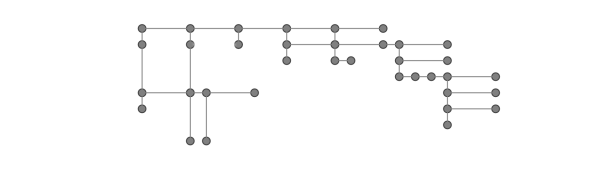
\includegraphics[width=0.8 \linewidth]{figure/nodeLink}
	\end{center}
	\caption{rappresentazione node-link HW drawing di un albero \label{fig:nodeLink}}
\end{figure}

Nella strategia Space-filling si tenta invece di superare i limiti del Node-link che riguardano la gestione non ottimale dello spazio orizzontale in quanto la parte alta della rappresentazione solitamente risulta essere poco densa di informazioni al contrario di quella bassa. Nella strategia Space-filling forme geometriche, solitamente rettangolari, rappresentano i nodi e i figli sono rappresentati da altre forme geometriche inserite all'interno del padre anche se anche questa rappresentazione presenta svariati problemi tra cui la distinzione difficile di tagli orizzontali da quelli verticali o la gestione non ottimale di alberi di grande profondità. Nella \textbf{\figurename~\ref{fig:spaceFilling}} sono mostrate alcune rappresentazioni diverse che seguono la strategia Space-filling.
\begin{figure}[!htb]
	\begin{center}
		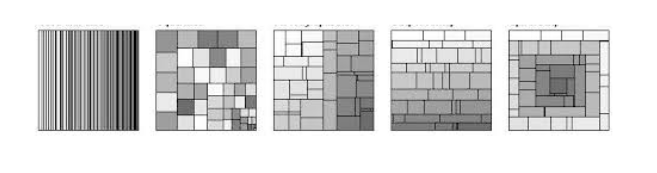
\includegraphics[width=0.9 \linewidth]{figure/spaceFilling}
	\end{center}
	\caption{rappresentazioni Space-filling\label{fig:spaceFilling}}
\end{figure}
\newline
Essendo quest'ultima di difficile lettura e soprattutto non ottimale per la rappresentazione di un albero collegato ad un grafo si è optato per la strategia Node-link scegliendo la rappresentazione "layered drawing",di cui ne è un esempio la \figurename{layered},in cui i nodi sono organizzati in livelli e per ogni nodo la coordinata y dipende dal livello mentre la coordinata x deve esser trovata e dipende dal numero di figli del livello e dello spazio orizzontale a disposizione per la rappresentazione.

\begin{figure}[!htb]
	\begin{center}
		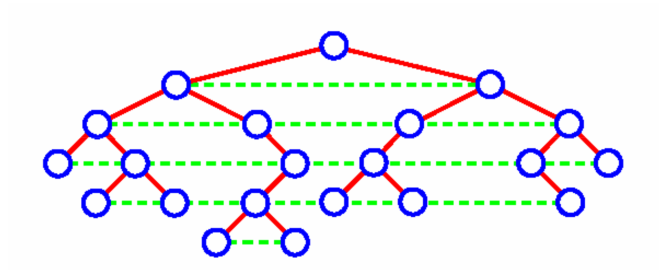
\includegraphics[width=0.9 \linewidth]{figure/layered}
	\end{center}
	\caption{rappresentazione node-Link layered Drawing\label{fig:layered}}
\end{figure}
\subsection{rappresentazione underlying Graph}
Avendo discusso della rappresentazione dell'inclusion Tree è necessaria la stessa attenzione per la rappresentazione dell'Underlying graph.  Essendo un albero un grafo orientato senza cicli i modelli di rappresentazione sono gli stessi visti per gli alberi. Il modello utilizzato è il \textbf{Force directed}, modello principale utilizzato per la visualizzazione di grafi che utilizza una rappresentazione Node-link, che fa in modo di emulare il sistema fisico formato da cariche elettriche rappresentate dai nodi e da molle rappresentati dagli archi. L'idea alla base del modello è quella che il raggiungimento di una condizione di equilibro corrisponda ad una rappresentazione grafica gradevole. ogni rappresentazione di un grafo è dunque formata da due componenti: il \textbf{modello} che descrive le forze in gioco e l'\textbf{algoritmo} ovvero la tecnica che permette di stabilire il punto di equilibrio accettabile. Ne esistono diverse varianti del modello Force directed e la scelta per quanto concerne il progetto in questone è ricaduta sul modello Spring Embedding, basato sulla combinazione di forze elettriche e forze meccaniche che andrà a formare una rappresentazione simile a quella mostrata nella \textbf{\figurename~\ref{fig:spring}}   
\begin{figure}[!htb]
	\begin{center}
		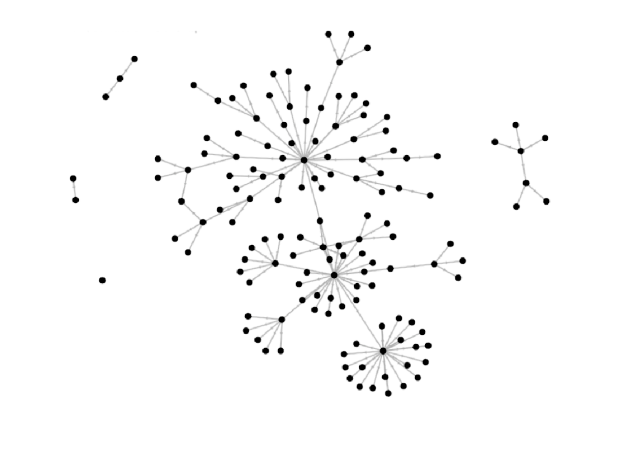
\includegraphics[width=0.8 \linewidth]{figure/spring}
	\end{center}
	\caption{rappresentazione Spring Embedding\label{fig:spring}}
\end{figure}
Per quanto concerne invece la complessità computazionale, il metodo non garantisce il numero di iterazione minimo per poter raggiungere una configurazione di equilibrio ed ogni passo iterativo ha complessità quadratica per i nodi e lineare per tutte le iterazioni avendo quindi un costo complessivo finale $O(n^3)$ senza lasciare però nessuna garanzia sul layout del grafo rappresentato.

\section{Linguaggi e librerie}
Avendo parlato della visualizzazione delle informazioni, è ancora da discutere su quale delle possibili tecnologie è stata utilizzata allo scopo della rappresentazione dinamica e user-friendly per poter creare l'editor.
Si è optato quindi per l'impiego di Javascript e della libreria D3.js che saranno viste nel dettaglio per motivazioni e punti di forza.
\subsection{Javascript}
JavaScript è un linguaggio di scripting orientato agli oggetti e agli eventi, comunemente utilizzato nella programmazione Web lato client. Essendo un sistema web con molti input da parte dell'utente a cui far fronte, Javascript consente un'ottima gestione di questi eventi. Le caratteristiche principali del linguaggio sono la debole tipizzazione, l'essere un linguaggio interpretato e non compilato con una sintassi relativamente simile a quella Java. Un altro punto a favore è la notevole facilità con cui si può lavorare con file con estensione .Json utilizzata proprio per l'import o l'export dei dati da rappresentare o della struttura dati della rappresentazione.
Un altro punto a favore è il supporto alla programmazione asincrona, cioè alla possibilità di eseguire attività in background che non interferiscono con il flusso di elaborazione principale, che per questo linguaggio risulta essere quasi una necessità essendo un linguaggio Single-threaded I due principali elementi che consentono di sfruttare il modello di programmazione asincrono in JavaScript sono gli eventi e le callback. Per completezza si vuol dare anche la definizione di programmazione asincrona come una forma di programmazione parallela che permette ad un’unità di lavoro di funzionare separatamente dal thread principale ed "avvertire" quando avrà finito l'esecuzione di quel task.\\
Si ricorda inoltre che un buon sistema deve essere documentato. Per questo è stata utilizzata \textbf{JsDoc}.
JSDoc è un generatore di documentazione per JavaScript, simile a Javadoc o phpDocumentor. Mediante l'aggiunta di commenti di documentazione all'interno del codice sorgente prima di ogni funzione o altro, JSDoc eseguirà la scansione del codice sorgente e generando un sito web HTML di documentazione. Essendo un sistema predisposto per l'utilizzo di potenziali utenti esperti è necessario dunque facilitare il riconoscimento del codice sorgente per modifiche e/o motivi di studio.
\subsection{D3.js}
A supporto della scelta dell'utilizzo del linguaggio di scripting javascript vi è l'utilizzo della libreria utilizzata per la visualizzazione delle informazioni D3.
D3.js (o solo D3 per Data-Driven Documents) è una libreria JavaScript per creare visualizzazioni dinamiche ed interattive partendo da dati organizzati, visibili attraverso un comune browser. Per fare ciò si serve largamente degli standard web: SVG, HTML5, e CSS.La libreria JavaScript D3, incorporata in una pagina web HTML, utilizza funzioni JavaScript per selezionare elementi del DOM, creare elementi SVG, aggiungergli uno stile grafico, oppure transizioni, effetti di movimento e/o tooltip. Questi oggetti possono essere largamente personalizzati utilizzando lo standard web CSS. In questo modo grandi collezioni di dati possono essere facilmente convertiti in oggetti SVG usando semplici funzioni di D3 e così generare ricche rappresentazioni grafiche di numeri, testi, mappe e diagrammi. 
Per completezza si ricorda che Scalable Vector Graphics abbreviato in SVG, indica una tecnologia in grado di visualizzare oggetti di grafica vettoriale e, pertanto, di gestire immagini scalabili dimensionalmente. 
Le figure espresse mediante SVG possono essere dinamiche e interattive. Il Document Object Model (DOM) per SVG, che include il completo XML DOM, consente una animazione in grafica vettoriale diretta ed efficiente attraverso il Javascript.
D3 consente dunque di associare dati arbitrari a un Document Object Model (DOM) e quindi applicare trasformazioni basate sui dati al documento per avere una manipolazione efficiente dei documenti basata sui dati. \\
Per completezza si specifica inoltre che il Document Object Model (DOM) è un'interfaccia multipiattaforma e indipendente dalla lingua che tratta un documento XML o HTML come una struttura ad albero come mostrato nella \textbf{\figurename~\ref{fig:dom}}   in cui ciascun nodo è un oggetto che rappresenta una parte del documento. Il DOM rappresenta un documento con un albero logico. Ogni ramo dell'albero termina in un nodo e ogni nodo contiene oggetti. I metodi DOM consentono l'accesso programmatico all'albero; con loro si può cambiare la struttura, lo stile o il contenuto di un documento. Ai nodi possono essere associati gestori di eventi. Una volta attivato un evento, i gestori degli eventi vengono eseguiti.
Un altro punto a favore dell'impiego di d3 e quindi di javascript riguarda le prestazioni. D3 è estremamente veloce, supporta set di dati di grandi dimensioni e comportamenti dinamici per l'interazione e l'animazione.
\begin{figure}[!htb]
	\begin{center}
		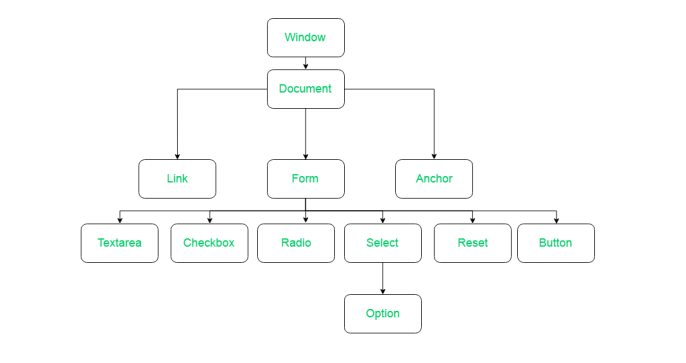
\includegraphics[width=0.8 \linewidth]{figure/dom}
	\end{center}
	\caption{rappresentazioni Space-filling\label{fig:dom}}
\end{figure}

\section{Oggetti per la struttura dati}
Inizialmente la struttura dati del progetto si basava su una unica struttura dati, in particolare un Array, contenente tutte le informazioni relative al c-Graph. La scelta è stata subito abbandonata a causa dei problemi riscontrabili con l'avere una struttura definibile quasi monolitica. Si è dunque passati ad una struttura ad oggetti ed in particolare si è scelto di utilizzare le strutture dello standard ECMAScript 6 quali map e set risultando essere una scelta migliore rispetto all'utilizzo di array per ragioni prestazionali, sicurezza e miglior accesso ai dati da rappresentare spesso senza bisogno di iterare completamente su tutti i valori indicizzati al loro interno. Inoltre risultano essere oggetti specializzati: il set garantisce l'unicità dei valori, la map conserva l'ordine di inserimento e non ha alcun legame con la prototype chain.Per completezza si ricorda inoltre che un oggetto Map è un oggetto che contiene coppie $<KEY,VALUE>$ in cui qualunque valore, sia esso oggetto o tipo primitivo, può esser usato come chiave e come valore. Ad avvalorare la scelta si nota che entrambi sono oggetti \textit{iterable} facili da iterare e i criteri di uguaglianza sulle chiavi della map sono più stretti di un normale $===$ e hanno funzionamenti e prestazioni migliori in caso di frequenti aggiunte o rimozioni di valori.
In particolare l'impiego degli oggetti sopra definiti e motivati nel caso in questione sarà discussa nel capitolo 4 in maniera molto approfondita.
}